\section{Debugging}

\subsection{Graph visualization}
A usefull way debug \gs applications is to generate visualizations of the pipeline.
This can be achieved by defining the environment variable \code{GST_DEBUG_DUMP_DOT_DIR} and executing the \code{GST_DEBUG_BIN_TO_DOT_FILE} macro on the final graph from the GStreamer application
\cite{johnstonGeneratingGStreamerPipeline2018}.
This will generate temprorary information information about the graph in \textit{.dot} files that can later be visualized using \gls{gviz}.
It's important to note that these graphs are not designed for print but rather for digital use, hence they tend to be very wide.

In Figure \ref{fig:gs_pipeline_visualization}, the visualized GStreamer graph used on the \sr is depicted.
The two red boxes on the left side represent the data received from the two cameras.
On the right side, there are six purple boxes corresponding to the three outputs for each camera.
These outputs include the \gls{h265} stream that is written to disk, the \gls{jpeg} photos (at a reduced framerate) that are sent to the \gls{gui}, and finally the raw frames used to verify the compression performance.
During normal operation, the raw outputs are disabled.

\begin{figure}[H]
    \centering
    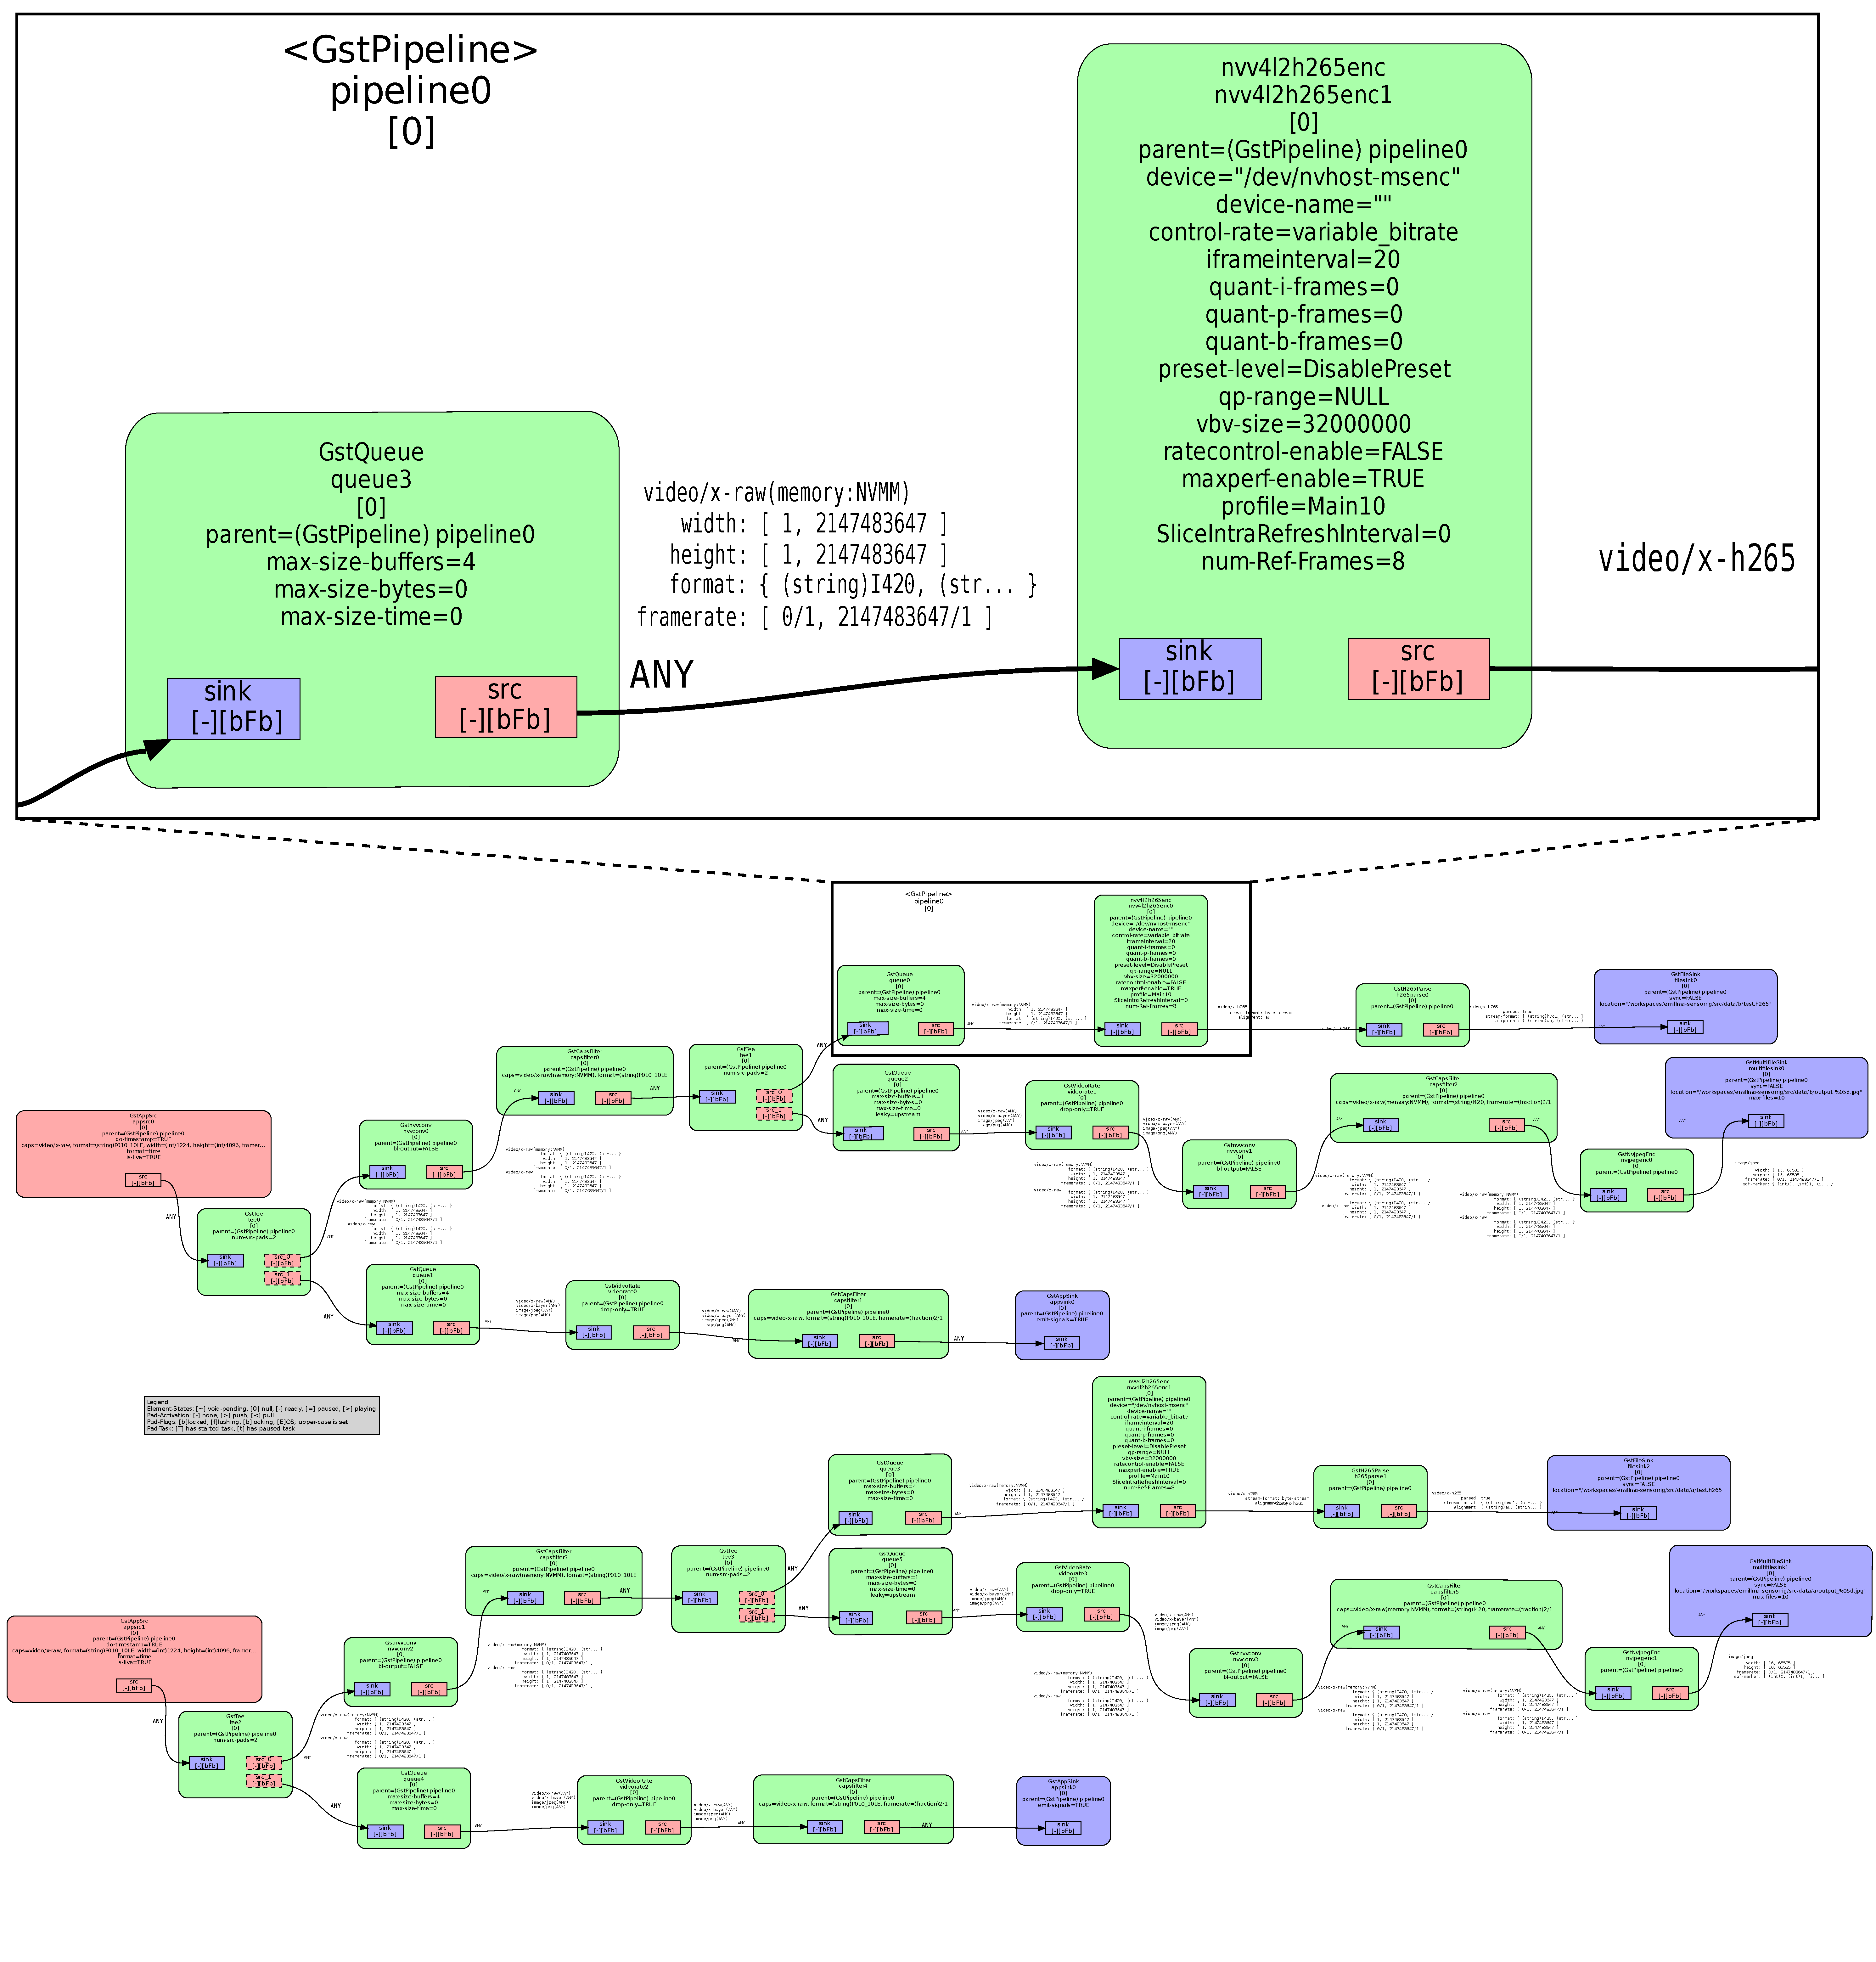
\includegraphics[width=\textwidth]{figures/gstreamer/gstreamer_pipeline.pdf}
    \caption{Visualization of the \gs Pipeline used on the \sr.
        The graph was crated using GraphViz and edited in Adobe Illustrator to be more compact.
        The top part shows a zoomed in version of the \gls{h265} encoder used on the second camera.}
    \label{fig:gs_pipeline_visualization}
\end{figure}

\subsection{Enabling Breakpoints in Callbacks}
It has been observed that the \gls{pygo} executes callbacks in separate threads.
However, it has been discovered that the default debugger in \gls{vscode}, Debugpy, ignores breakpoints in these threads \cite{microsoftDebugpyDebuggerPython2023}\cite{visualstudiocodeDebuggingConfigurationsPython2023}.
To enable debugging in these threads, it is necessary to manually call \code{debugpy.debug_this_thread} at the beginning of the callback function \cite{nadigAnswerDebugNot2019}.
With debugging enabled it is possible to halt the execution and inspect the current state of the graph.
This is especially usefull in combination with \gls{gstreamer} probes that can be attached to any pad in the graph, making it possible to inspect the data flowing through the pipeline \cite{gstreamerProbes}.


\subsection{Inspection and Comparison of the Final Output}
\label{sec:inspection_and_comparison_of_the_final_output}
Examining the output is another effective way to verify the proper functioning of the pipeline and detect potential issues related to different image formats.

One specific issue that was resolved through this type of debugging was the detection of a mismatch between the color profile used in the H.265 encoder and the one used in the color space conversion in \gls{cuda}.
Although the compressed video output appeared visually accurate with no visible artifacts, the calculated noise-to-signal ratios indicated a problem.
By subtracting the original frame from the decompressed frame and adding 512 to avoid underflow, an error image with a distinct pattern emerged, as depicted in Figure \ref{fig:compression_error}.
The error image showed that where the original image was bright, the error image was dark, and vice versa.
This observation indicated that the compressed video could not reproduce the brightest or darkest colors from the original video.
It was quickly recognized that the encoder was probably was utilizin another color profile, specifically bt.601 instead of bt.709.
While exact documentation confirming this discrepancy could not be found, after re-implementing the \cuda implementation to utilize bt.601, the noise-to-signal ratios decreased significantly and the error pattern disappeared.

\begin{figure}
    \centering
    \subcaptionbox{Original frame.}{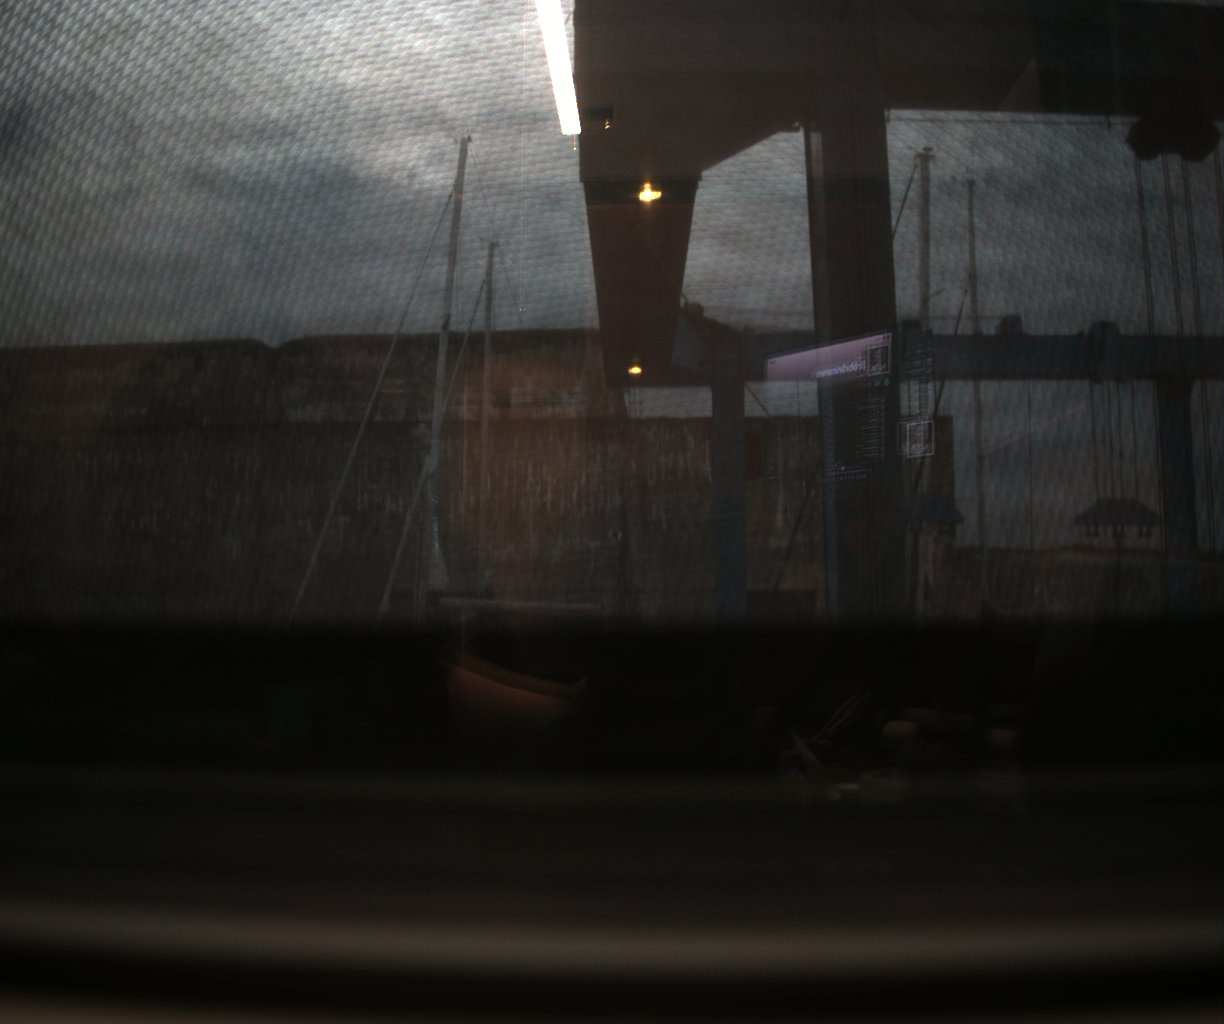
\includegraphics[width=0.48\textwidth]{figures/compression/error_orig.jpg}}
    \subcaptionbox{Original frame subtracted from the decompressed frame.
        Constant added to avoid underflow.
    }{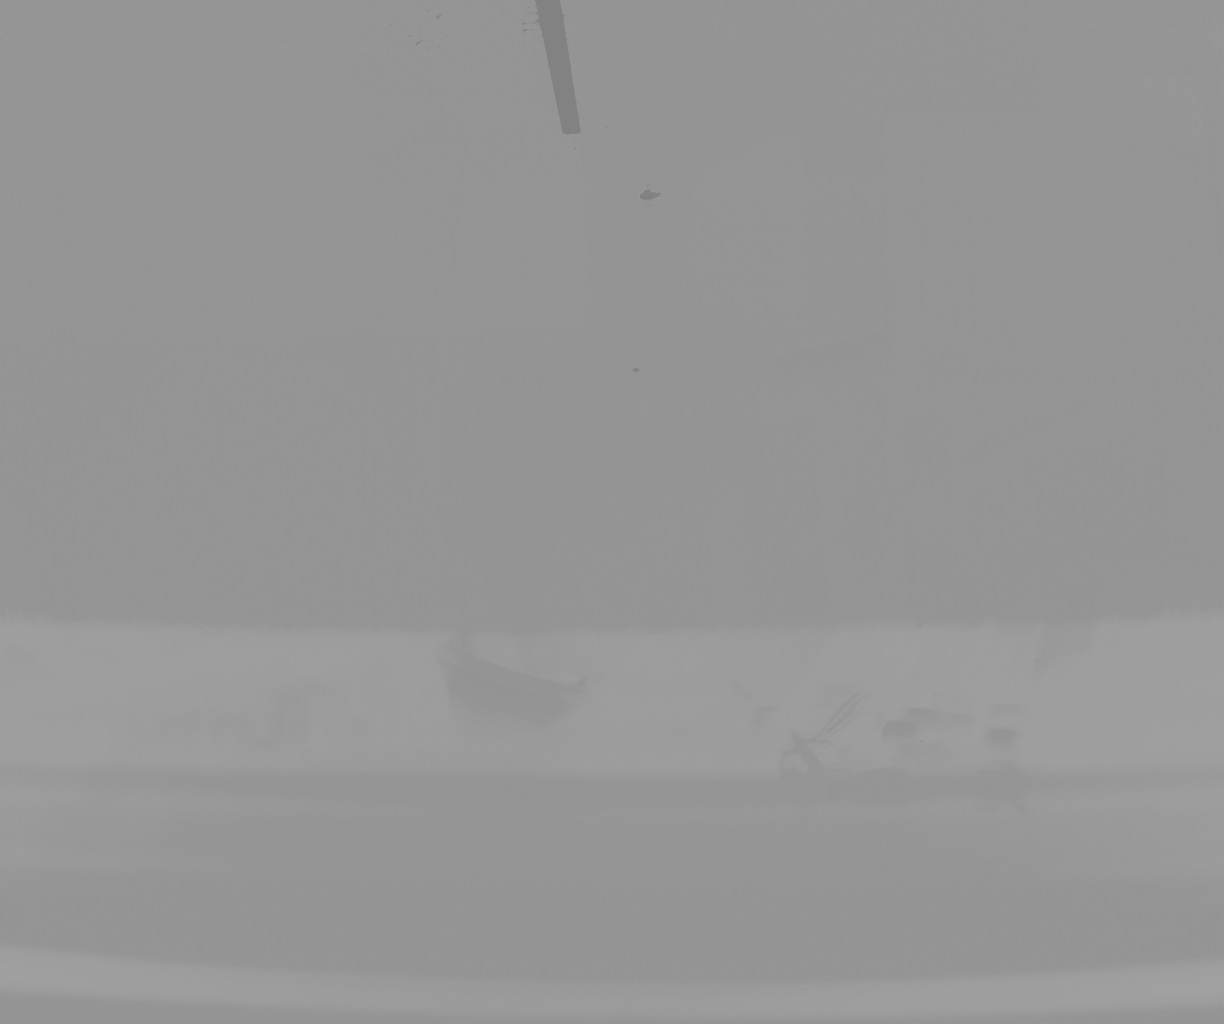
\includegraphics[width=0.48\textwidth]{figures/compression/error_error.jpg}}
    \caption{Original frame and compression error revealing use of wrong color profile as brigh regions are too dark and dark regions are too bright.}
    \label{fig:compression_error}
\end{figure}